\section{Graphical Design}
In graphical design, like any other design, there are many options to be considered. Colours, fonts, balance and many more factors should be chosen carefully. Most importantly, how to mix these elements together without making a mess. 
This will reflect greatly on how a design is being perceived. \cite{ColorMeaning}

Two of the things people often complaint about in applications is a confusing interface design and poor navigation. \cite{Pattern} This can be prevented by using design patterns. These has been created to avoid a messy and untolerable app.
First, navigation. There are two ways to make navigating through an app easier. Persistent and transient. Persistent navigation is list menus and tab menus or menu structures. Transient navigation has to be revealed through a tab action or the likes.\cite{Pattern}
Consider if the user needs to see the menu at all times and if not, an off-canvas solution like a side-bar could be preferred.\cite{Pattern} This way, the app is able to hold many informations without being confusing or plastered.  
Too much text in one page or a simple form taking up several pages will make the app confusing. A sign in for example should only be one page. A way to not get an over lapping look is by using vertical labels instead of horizontal. \cite{Pattern} Or you could have the horizontal labels where the text disappears as soon as the user starts typing, but you risk that the user forgets what they should fill in.\cite{Pattern} 
Some apps, like Instagram, shows the "sign in" and "sign up" option all the way through the tutorial. This also insures that the user do not have to go through a whole tutorial if they do not need it. 

Keeping these patterns in mind there are still many things to consider. 
First of all, remember the size of the screen that is being designed for. Avoid using big scaled photos and put to much information on one page. This will make it look cluttered and make it less intuitive. \cite{Sardo}
In short, make everything as clean and simple as possible. 

\subsubsection{Colors}

Colours are not just colours when designing a brand, an app or a website. Colours are perceived in various ways and is a big part of how the design is coming  across to the user. \cite{ColorMeaning}

It is important to remember that when choosing the colour palette for a design, that how we perceive colour is very different. Also, colours can change according to what it is next to. Yellow might look different next to grey than it will next to purple for instance. \cite{Colour}

When it comes to colour psychology the truth is, it is too dependent on personal experience. There is no one right answer to which color falls into what mood. \cite{ColorMeaning}
There is, however, many studies conducted on this matter. 
One study shows that 90\% of people make snap judgement based on colour alone. \cite{ColorMeaning} Another study shows that an intend of purchasing is linked with how a brand is perceived i.e. what kind of "personality" does the brand have?\cite{ColorMeaning}

\begin{figure}[H]
\centering
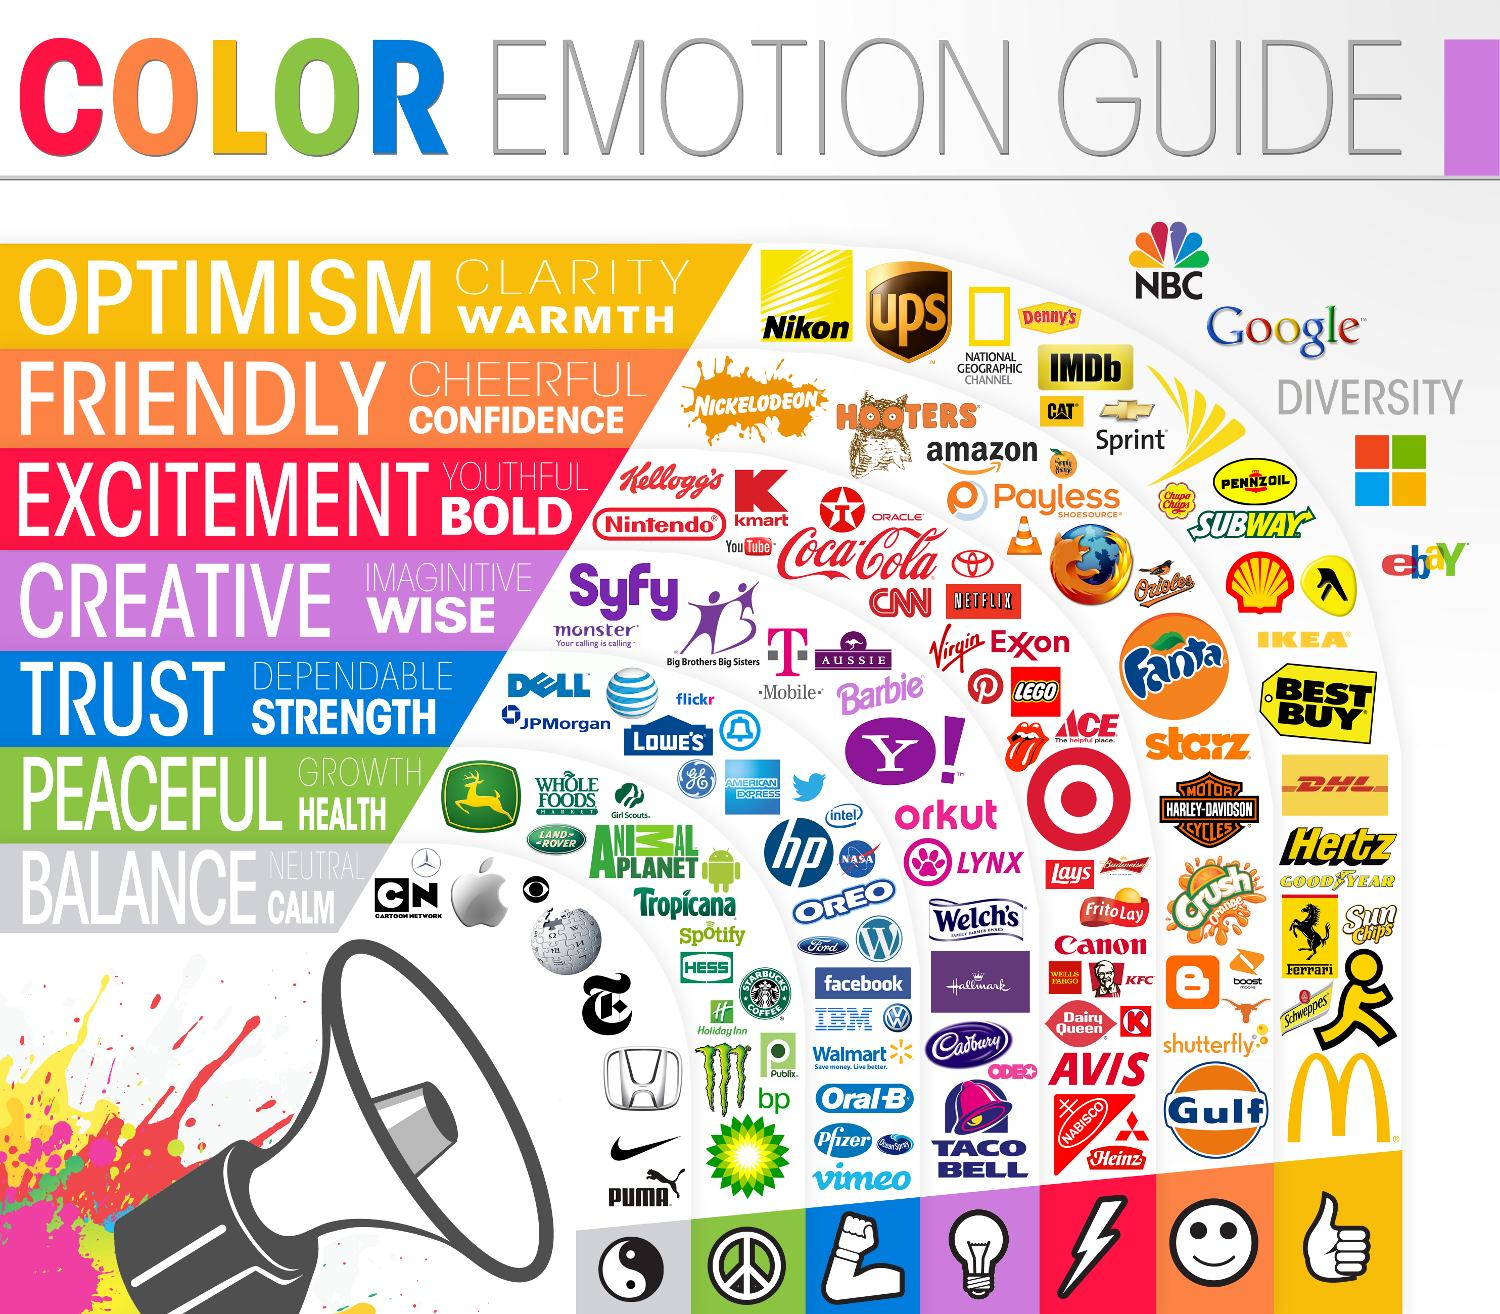
\includegraphics[scale=0.125]{color-emotion.jpg}
\caption{Overall image of how colours are generally percieved. \cite{ColorMeaning}}
\end{figure}

But all in all, the concept of the app is key. Almost every study shows that it is greatly more important to choose a colour that shows the personality of your product than picking a stereotype colour. \cite{ColorMeaning} This app is directed towards interior design and therefore it is fitting to give the app a inspiring and creative personality. According to fig. 2.12 the color purple is the inspirational and creative color. This is very feminine but mixing it with a neutral colour like grey might just take it down a notch. %check fig. number

Colour preferences differ between genders as well. A study shows that women prefer soft colours and tints while men prefer bright colours and shades. \cite{ColorMeaning} Since the target group of this app is not gender specific it is important to make the app gender-neutral i.e. not to soft and feminine but at the same time not to bright. 

So how does one find the best way to coordinate different colours? Research indicates that the isolation effect is very useful.

\begin{figure}[H]
\centering

\includegraphics[scale=0.5]{isolation_effect.png}
\caption{"The sign-up button stands out because it's like a red "island" in a sea of blue." \cite{ColorMeaning}}
\end{figure}

Using the isolation effect will help the user have a more efficient experience because the most important feature e.g. a "sign up" button, stands out. \cite{ColorMeaning} (See fig. 2.13)%remember too look this after later on
Research suggests that a colour scheme that consists of analogues colors and combine it with a accent complimentary color or a tertiary color is preferred among users. \cite{ColorMeaning} 

When designing your layout it is, once again, key to keep everything simple and streamlined. 
Follow the general rules, left-to-right and top-to-bottom. Make sure the most important feature is in the top left corner where the user will look first.\cite{Sardo}
Be careful, yet not boring, when choosing a colour scheme or font type. 
In general, keep the graphics clean and simple. No muss, no fuss. 